\chapter{The small current element: Hertz dipole}
Let us consider the simplest case of the current distribution which is a small current element of infinitesimally small elements $d\vec{l}$ whose direction is specified by the direction in which the current flows. This current distribution is the smallest current distribution possible and any other current distribution is the superposition of this small element. The choice of a small current element gives the foundation for finding electric and magnetic fields for any arbitrary current distribution.

The small current element is also referred to as the \emph{Hertz dipole}\index{hertz dipole} which is characterized by what is called the \emph{current moment}\index{current moment}. The current moment is the product of the current and the length of the element, $Id\vec{l}$. For the current distribution, we assume a sinusoidally varying time-varying function for our analysis such that $I = I_0d\vec{l}e^{j\omega t}$. This current element can be imagined as a small rod of the cross-sectional area which carries $\vec{J}$ such that the integral over the cross-sectional area gives the current which is multiplied by the length of the rod, $d\vec{l}$, to give the current moment. Hence $\int_v\vec{J}dv' = I_0d\vec{l}e^{j\omega t}$ (with the assumption that the current is constant across the length of the rod, $d\vec{l}$). 

Now, we will determine the vector potential $\vec{A}$ at some point in space given by $(r, \theta, \phi)$ in the spherical coordinate system, as shown in Figure~\ref{fig:small_current_element}. It shows the current element of length, $d\vec{l}$ at the origin.
\begin{figure}[h]
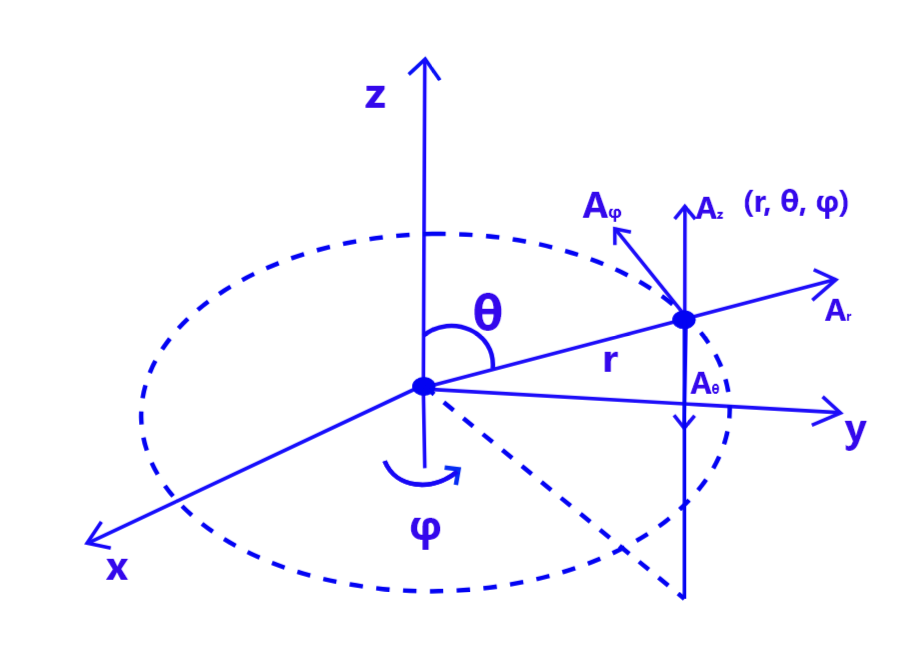
\includegraphics[width=0.8\linewidth]{\pathtoparttwo/graphics/fig1_1}
\centering
\caption{Analysis of a small current element in the spherical coordinate system}
\label{fig:small_current_element}
\end{figure}

We recall that the vector potential given in equation~\eqref{eqn:vector_potential_complete}, we substitute r for $|\vec{r} - \vec{r'}|$ because $\vec{r'}$ is the position where the current element is located which is the origin such that the vector potential is;
\begin{align}
\vec{A}(\vec{r}) =\int_v \frac{\mu \vec{J}(\vec{r'}) e^{-j\beta r}}{4\pi r}dv'
\label{eq:vector_potential_lec48}
\end{align} 
Also since the length of the current element is much smaller compared to $r$, then $\frac{e^{-j\beta r}}{4 \pi r}$ is practically constant and the vector potential can be written as;
\begin{dmath*}
\vec{A}(\vec{r}) = \frac{\mu e^{-j\beta r}}{4 \pi r}\int_v\vec{J}(\vec{r'})dv'
= \frac{\mu I d\vec{l} e^{-j\beta r}}{4\pi r},\quad\text{Recall, }I\text{ = }I_0e^{j\omega t}
\end{dmath*}
From the expression above it can be seen that the direction of the vector potential is determined by the direction of $d\vec{l}$ and $d\vec{l}$ is oriented in the $z$ direction. 
\begin{dmath*}
\vec{A} = A_z\hat{z}
= \frac{\mu I_0 e^{j\omega t} dl e^{-j\beta r}}{4\pi r}\hat{z}
\end{dmath*}
But we want our analysis to be done in the spherical coordinate system $(r, \theta, \phi)$. So we will convert from the $z$ direction to the $(r, \theta, \phi)$ direction. However, the $z$ direction has components in the $r$ and $\theta$ direction only because the $\phi$ direction is perpendicular to the $z$ direction. The component $A_{r}$ and $A_{\theta}$ are given as;
\begin{align*}
A_{r} = A_z\cos\theta\quad A_{\theta} = - A_z\sin\theta\quad A_{\phi} = 0
\end{align*}
Now, with the vector potential that has been determined, we would find out the magnetic field through the relationship $\mu \vec{H} = \nabla \times \vec{A}$ (since $\vec{B} = \nabla \times \vec{A}$ and $ \vec{B} = \mu \vec{H}$)
\begin{dmath*}
\vec{H} = \frac{1}{\mu} \nabla \times \vec{A} = \frac{1}{r^2\sin\theta}
\begin{vmatrix}
\hat{r} & r\hat{\theta} & r\sin\theta\hat{\phi} \\
\partialderivative{}{r} &  \partialderivative{}{\theta} &  \partialderivative{}{\phi} \\
A_r & rA_{\theta} & r\sin\theta A_{\phi}
\end{vmatrix}
\end{dmath*}
For the analysis, there is $r$ and $\theta$ dependence because the vector $\vec{A}$ is a function of $r$ and in the $\theta$ direction the source would not appear the same that is at $\theta = 0$, we see the top of the current element while when $\theta = \frac{\pi}{2}$ we see a line. But in the $\phi$ direction, the source is symmetrical so there is no $\phi$ dependence.

Hence, 
\begin{dmath*}
\vec {H} = \frac{1}{\mu r^2\sin\theta}
\begin{vmatrix}
\hat{r} & r\hat{\theta} & r\sin\theta\hat{\phi} \\
\partialderivative{}{r} &  \partialderivative{}{\theta} &  0 \\
A_r & rA_{\theta} & 0
\end{vmatrix}
= 0 \hat{r} - 0\hat{\theta} + \frac{r\sin\theta}{\mu r^2\sin\theta}\hat{\phi}\left( \frac{\partial }{\partial r}(rA_{\theta}) - \frac{\partial }{\partial \theta} A_r\right)
= \frac{\hat{\phi}}{\mu r}\left(\frac{\partial}{\partial r}(r(-A_z sin\theta)) - \frac{\partial}{\partial \theta}(A_z cos\theta)\right)\footnotemark
= \frac{\hat{\phi}}{\mu r} \left(-sin\theta\left(r\frac{dA_z}{dr} + A_z\right) - A_z \frac{d(cos\theta)}{d\theta}\right)
= -\frac{\hat{\phi}}{\mu r} (\sin\theta\left(r\frac{dA_z}{dr} + A_z\right) - A_zsin\theta)
= -\frac{\sin\theta\hat{\phi}}{\mu r} \left(r\frac{dA_z}{dr} + A_z - A_z\right)
= -\frac{\sin\theta\hat{\phi}}{\mu } \frac{dA_z}{dr}
\end{dmath*}
\footnotetext{
Recall that $A_z$ is a function of $r$
}
Recall that $A_z = \frac{\mu I_0 e^{j\omega t} dl e^{-j\beta r}}{4\pi r}$
So,
\begin{dmath*}
\frac{dA_z}{dr} = \frac{\mu I_0 e^{j\omega t} dl}{4\pi}\derivative{}{r}\left(\frac{e^{-j\beta r}}{r}\right)
= \frac{\mu I_0 e^{j\omega t} dl}{4\pi} \left(\frac{r(-j\beta e^{-j\beta r}) - e^{-j\beta r}}{r^2}\right)
= \frac{\mu I_0 e^{j\omega t}e^{-j\beta r} dl}{4\pi}  \left(\frac{-jr\beta - 1}{r^2}\right)
= - \frac{\mu I_0 e^{j\omega t}e^{-j\beta r} dl}{4\pi} \left(\frac{jr\beta}{r^2} + \frac{1}{r^2}\right)
= - \frac{\mu I_0 e^{(j\omega t-j\beta r)} dl}{4\pi} \left(\frac{j\beta}{r} + \frac{1}{r^2}\right)
\end{dmath*}
Hence,
\begin{equation}
\vec{H} = \frac{\sin\theta I_0 dl e^{j(\omega t-\beta r)} }{4\pi} \left(\frac{j\beta}{r} + \frac{1}{r^2}\right)\hat{\phi}
\label{eqn:magneticfieldsmallcurrentelement}
\end{equation}
With the magnetic field, we apply Maxwell's equation to find the electric field at a location in space where there is no charge or no source. So, we can substitute the magnetic field in the source-free Maxwell's equation given by $\nabla \times \vec{H} = j\omega \epsilon\vec{E}$ from the wave equations.
\begin{align*}
\vec{E} = \frac{1}{j\omega \epsilon}\nabla \times \vec{H}
\end{align*}
Also analyzing the electric field equation in the spherical coordinate system, 
\begin{dmath*}
\vec{E}  = \frac{1}{j\omega \epsilon} \times \frac{1}{r^2sin\theta}
\begin{vmatrix}
\hat{r} & r\hat{\theta} & r\sin\theta\hat{\phi} \\ 
\frac{\partial}{\partial r} & \frac{\partial}{\partial \theta} &  \frac{\partial}{\partial \phi} \\
H_r & rH_\theta & r\sin\theta H_\phi              
\end{vmatrix}
\end{dmath*}
The magnetic field vector, $\vec{H}$ which we got has only the $\phi$ component and it is dependent on $r$ and $\theta$ only so the expression simplifies to 
\begin{dmath*}
\vec{E}  = \frac{1}{j\omega \epsilon} \times \frac{1}{r^2sin\theta}
\begin{vmatrix}
\hat{r} & r\hat{\theta} & r\sin\theta\hat{\phi} \\ 
\frac{\partial}{\partial r} & \frac{\partial}{\partial \theta} &  0 \\
0 & 0 & r\sin\theta H_\phi              
\end{vmatrix}
\end{dmath*}
\begin{dmath*}
\vec{E}  = -\frac{j}{\omega \epsilon r^2sin\theta}
\begin{vmatrix}
\hat{r} & r\hat{\theta} & r\sin\theta\hat{\phi} \\ 
\frac{\partial}{\partial r} & \frac{\partial}{\partial \theta} &  0 \\
0 & 0 & r\sin\theta H_\phi              
\end{vmatrix}  = \frac{-j}{\omega  \epsilon r^2\sin\theta}\left(\hat{r} \frac{\partial}{\partial \theta}\left(r\sin \theta H_{\phi}\right) - r\hat{\theta} \frac{\partial}{\partial r}(r\sin\theta H_{\phi}) + 0\hat{\phi}\right)
= \frac{-j \hat{r}}{\omega \epsilon r^2\sin\theta}\frac{\partial}{\partial \theta}(r\sin\theta H_{\phi}) + \frac{j \hat{\theta}}{\omega  \epsilon r\sin\theta}\frac{\partial}{\partial r}(r\sin\theta H_{\phi})
= \frac{-j \hat{r}}{\omega  \epsilon r\sin\theta}\frac{\partial}{\partial \theta}(\sin\theta H_{\phi}) + \frac{j \hat{\theta}}{\omega  \epsilon r}\frac{\partial}{\partial r}(r\sin\theta H_{\phi})
= \frac{-j \hat{r}}{\omega \epsilon r\sin\theta}\left(\sin\theta\frac{\partial }{\partial \theta}H_{\phi} + H_{\phi}\frac{d\sin\theta}{d\theta}\right) + \frac{j\hat{\theta}}{\omega \epsilon r}\left(r\frac{\partial}{\partial r}H_{\phi} + H_{\phi}\right)
\end{dmath*}
Comparing the above equation with $\vec{E} = E_r\hat{r} + E_{\theta}\hat{\theta}$, then we have the electric field components as
\begin{dmath*}
E_r = \frac{-j \hat{r}}{\omega \epsilon r\sin\theta}\left(\sin\theta\frac{\partial }{\partial \theta}H_{\phi} + H_{\phi}\frac{d\sin\theta}{d\theta}\right)
= \frac{-j}{\omega \epsilon r}\frac{\partial}{\partial \theta}H_{\phi} - \frac{j\cos\theta}{\omega \epsilon r\sin\theta}H_\phi
\end{dmath*}
Recall that $H_{\phi} = \dfrac{\sin\theta I_0 dl e^{j(\omega t-\beta r)} }{4\pi} \left(\dfrac{j\beta}{r} + \dfrac{1}{r^2}\right)$ from equation~\eqref{eqn:magneticfieldsmallcurrentelement}
\begin{dmath*}
\dfrac{\partial H_{\phi}}{\partial \theta} =  \frac{I_0 dl e^{j(\omega t-\beta r)} }{4\pi} (\frac{j\beta}{r} + \frac{1}{r^2})\dfrac{d (\sin\theta)}{d \theta}
= \dfrac{\cos \theta I_0 dl e^{j(\omega t-\beta r)} }{4\pi} \left(\frac{j\beta}{r} + \frac{1}{r^2}\right)
\end{dmath*}
So, the radial component of the electric field is
\begin{dmath*}
E_r =  \frac{-j}{\omega \epsilon r}\left(\frac{\cos \theta I_0 dl e^{j(\omega t-\beta r)} }{4\pi} \left(\frac{j\beta}{r} + \frac{1}{r^2}\right)\right) -  \frac{j\cos\theta}{\omega \epsilon r\sin\theta}\frac{\sin\theta I_0\vec{dl} e^{j(\omega t-\beta r)} }{4\pi} \left(\frac{j\beta}{r} + \frac{1}{r^2}\right)
= \frac{\cos \theta I_0 dl e^{j(\omega t-\beta r)} }{4\pi \omega  \epsilon} \left(\frac{\beta}{r^2} - \frac{j}{r^3}\right) + \frac{\cos \theta I_0 dl e^{j(\omega t-\beta r)} }{4\pi \omega \epsilon} \left(\frac{\beta}{r^2} - \frac{j}{r^3}\right)
= \frac{2\cos \theta I_0 dl e^{j(\omega t-\beta r)} }{4\pi \omega\epsilon} \left(\frac{\beta}{r^2} - \frac{j}{r^3}\right)
\end{dmath*}
Therefore,
\begin{equation}
E_r = \frac{\cos \theta I_0 dl e^{j(\omega t-\beta r)} }{2\pi \omega \epsilon} \left(\frac{\beta}{r^2} - \frac{j}{r^3}\right)
\label{eqn:electricfieldradialcomponentsmallcurrentelement}
\end{equation}
Also,
\begin{dmath*}
E_{\theta} = \frac{j}{\omega\epsilon r}\left(r\frac{\partial}{\partial r}H_{\phi} + H_{\phi}\right)
=  \frac{j}{\omega \epsilon}\frac{\partial H_{\phi}}{\partial r} + \frac{j}{\omega \epsilon r}H_{\phi}
\end{dmath*}
Then,
\begin{dmath*}
\frac{\partial H_{\phi}}{\partial r} = \frac{\sin \theta}{4 \pi} I_0 dl \derivative{}{r}\left(e^{j(\omega t - \beta r)}\left(\frac{j \beta}{r} + \frac{1}{r^2}\right)\right) = \frac{\sin \theta}{4 \pi} I_0 dl \left(e^{j(\omega t - \beta r)}\left(\frac{-j\beta}{r^2} - \frac{2}{r^3}\right) + (-j\beta)e^{j(\omega t - \beta r)}\left(\frac{j \beta}{r} + \frac{1}{r^2}\right)\right)
= \frac{\sin \theta}{4 \pi} I_0 dle^{j(\omega t - \beta r)} \left(\frac{-j\beta}{r^2} - \frac{2}{r^3} + \frac{\beta^2}{r} - \frac{j\beta}{r^2}\right)
= \frac{\sin \theta}{4 \pi} I_0 dle^{j(\omega t - \beta r)} \left( \frac{\beta^2}{r} - \frac{2}{r^3}  - \frac{j2\beta}{r^2}\right)
\end{dmath*}
So,
\begin{dmath*}
E_{\theta} =  \frac{j}{\omega\epsilon}\frac{\sin \theta}{4 \pi} I_0 dle^{j(\omega t - \beta r)}\left( \frac{\beta^2}{r} - \frac{2}{r^3}  - \frac{j2\beta}{r^2}\right) + \frac{j}{\omega \epsilon r}\frac{\sin\theta I_0\vec{dl} e^{(j\omega t-j\beta r)} }{4\pi} \left(\frac{j\beta}{r} + \frac{1}{r^2}\right)
= \frac{I_0sin \theta dl e^{j(\omega t - \beta r)}}{4\pi \omega\epsilon}\left(\frac{j\beta^2}{r} - \frac{j2}{r^3} + \frac{2\beta}{r^2} - \frac{\beta}{r^2} + \frac{j}{r^3}\right)
\end{dmath*}
Therefore the $\theta$ component of the electric field is
\begin{equation}
E_{\theta} = \frac{I_0sin \theta dl e^{j(\omega t - \beta r)}}{4\pi \epsilon}\left(\frac{j\beta^2}{\omega r} + \frac{\beta}{\omega r^2} - \frac{j}{\omega r^3}\right)
\label{eqn:electricfieldthetacomponentsmallcurrentelement}
\end{equation}
Now we note that the magnetic field of the hertz dipole is oriented in the $\phi$ direction around the $z$ axis while the electric field has two components\textemdash one in the $r$ direction which is the $r$ component and one in the $\theta$ direction which is the $\theta$ component.

\section{Near and Far fields}
A few important points emerge when studying equations~\eqref{eqn:magneticfieldsmallcurrentelement}, ~\eqref{eqn:electricfieldradialcomponentsmallcurrentelement} and~\eqref{eqn:electricfieldthetacomponentsmallcurrentelement}, a careful look shows the expressions contain terms varying with $\frac{1}{r^3}$, $\frac{1}{r^2}$ and $\frac{1}{r}$. At points very close to the current element, the  $\frac{1}{r^3}$ term must be dominant. The variation of an electric field with  $\frac{1}{r^3}$ should remind us of the electrostatic field of the dipole. The near field terms of  $\frac{1}{r^3}$ in the electric field component represent energy stored in a reactive (capacitive) field and they do not contribute to the radiated power. Also, the  $\frac{1}{r^2}$ term in the $H_\phi$ expression is similarly important only in the region very near to the current element. It corresponds to the induction field of the DC element as found through Biot-Savart law. At a distance far away from the source, the effect of the  $\frac{1}{r^3}$ and  $\frac{1}{r^2}$ terms reduces drastically except for the effect of the  $\frac{1}{r}$ term, and we are said to be in the far-field zone. Thus the remaining fields that have the  $\frac{1}{r}$ dependence are the radiation fields. 

Let's take a look at equation ~\eqref{eqn:electricfieldthetacomponentsmallcurrentelement}, the term $\frac{\beta^2}{\omega r}$ can be further simplified to $\frac{\omega \mu \epsilon}{r}$, which means it varies inversely with r and is proportional to the frequency,$\omega$. Also considering the $\frac{\beta}{\omega r^2}$ term, substituting $\beta = \omega \sqrt{\mu \epsilon}$ gives $\frac{\sqrt{\mu \epsilon}}{r^2}$ which is independent of the frequency, $\omega$ and the term $\frac{1}{\omega r^3}$ term (the \emph{electrostatic field}\index{electrostatic field}), varies as $\frac{1}{\omega }$. Hence at lower frequencies the $\frac{1}{\omega r^3}$ dominates while at higher frequencies the $\frac{\beta^2}{\omega r}$ dominates for the same current $I_0dl$ which tallies with the statement established earlier that frequency increases the radiation increases. 

Let's better explain the electrostatic fields; it has been established that at lower frequencies this field dominates. For it to be called an electrostatic field there must be charges but in our analysis, we did not introduce charges, all we introduced was a current element where we assumed there is a current $I$ flowing through it. However, a new question is asked \emph{where does the current go?} Current is the flow charge and we are considering time-varying currents, so for half a cycle the flow of the current is upward while in the second half, the flow is downward. Considering the first half cycle the flow of current causes the accumulation of positive charges at the top and negative charges at the bottom as shown in Figure~\ref{fig:dipole}(a).
\begin{figure}[h]
\centering
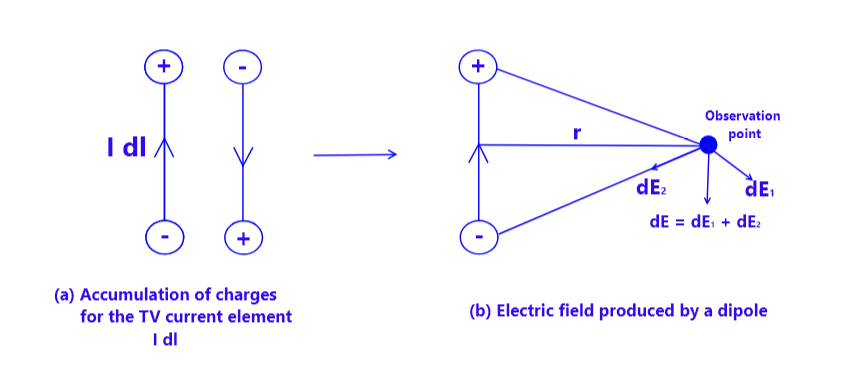
\includegraphics[width=1\linewidth]{\pathtoparttwo/graphics/fig1_2}
\caption{(a) Accumulation of charges at the top and bottom of the current element (b) Electric field at an observation point a distance r from the dipole}
\label{fig:dipole}
\end{figure}

For the next half cycle, the accumulation of positive charges occurs at the bottom while the negative charges are accumulated at the top since the current is flowing downwards. So essentially, this current flow which is time-varying is equivalent to having time-varying charges that can be likened to an electric dipole whose charges are changing as a function of time. Considering a condition for a half cycle and calculating the electric field at an observation point a distance r from the dipole as shown in Figure~\ref{fig:dipole}(b), gives an electric field which varies with $\frac{1}{r^3}$.

Now the next question to ask is \emph{why does this field dominate at a lower frequency?} Well, we know that charge is the integral of current over time i.e. $Q =\int Idt$, so for a period which is very large for the same current amplitude the accumulated charges would be more. So as frequency goes on reducing the amount of charge that will get accumulated will increase. This is why at lower frequencies the electrostatic field dominates.

Essentially, there are 3 fields; \emph{the electrostatic field}, \emph{the induction field} and \emph{the radiation field}, which are generated by the simple Hertz dipole. Our interest however is the radiation field. 

From equation~\eqref{eqn:electricfieldthetacomponentsmallcurrentelement}, let $E_{\theta} = 0$. Thus,
\begin{align*}
&\frac{j\beta^2}{\omega r} + \frac{\beta}{\omega r^2} - \frac{j}{\omega r^3} = 0&\\
&\text{Taking the modulus}&\\
&\frac{\beta^2}{\omega r} + \frac{\beta}{\omega r^2} - \frac{1}{\omega r^3} = 0&\\
&\text{Multiply through by $\omega$}&\\
&\frac{\beta^2}{r} + \frac{\beta}{r^2} - \frac{1}{r^3} = 0&\\
&\text{Multiply through by $r^3$}&\\
&(r\beta)^2 + r\beta - 1 = 0&\\
&(r\beta)^2 + r\beta = 1&\\
&r\beta(r\beta + 1) = 1&\\
&r\beta = 1\quad\text{ or }\quad r\beta + 1 = 1&\\
&r = \frac{1}{\beta}\quad\text{ or }\quad r = 0&\\
\end{align*}
Since at $ r = 0$, the expression in equation~\eqref{eqn:electricfieldthetacomponentsmallcurrentelement} becomes undefined, then $ r = \frac{1}{\beta} $; $\beta = \frac{2\pi}{\lambda} \Longrightarrow r =  \frac{\lambda}{2 \pi} $.

At $ r =  \frac{\lambda}{2 \pi} $ the Electric field goes to zero and the plot is given in Figure~\ref{fig:electricfiedvariationwithdistance}.
\begin{figure}[h]
\centering
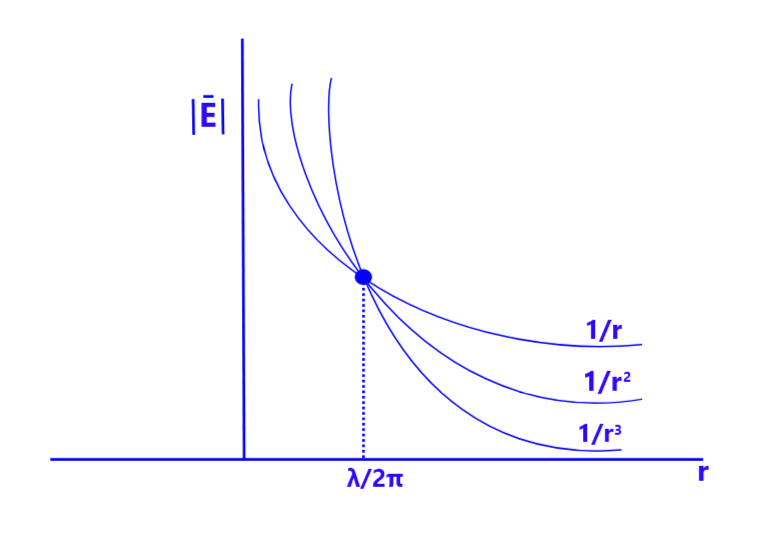
\includegraphics[width=0.7\linewidth]{\pathtoparttwo/graphics/fig1_3}
\caption{Variation of the electric field with distance}
\label{fig:electricfiedvariationwithdistance}
\end{figure}

Using the distance $r =  \frac{\lambda}{2 \pi}$ as the reference point and with this we will classify these fields into two categories;
\begin{enumerate}[(i)]
\item At $r \ll  \frac{\lambda}{2 \pi}$, we have the near fields.
\item At $r \gg  \frac{\lambda}{2 \pi}$, we have the far fields.
\end{enumerate}
The near fields consist of the three fields and as such consists of the 3 components; $E_r$, $E_{\theta}$, and $H_{\phi}$. While the far fields would consist of the radiation fields alone since every other field is negligible at the far field zone, so the far fields contain the $E_\theta$ and $H_\phi$ components only.
\begin{align}
E_{\theta} &= j\frac{I_0sin \theta dl\beta^2 e^{j(\omega t - \beta r)}}{4\pi \omega \epsilon r}\label{eqn:electricfarfield}\\
H_\phi &= j\frac{I_0 dl \beta \sin\theta   e^{(j\omega t-j\beta r)} }{4\pi r}\label{eqn:magneticfarfield}
\end{align}
For the far fields which are our interest, we would note a few important points;
\begin{enumerate}[(i)]
\item Both fields vary as a function $\theta$ (they both contain $sin\theta$) which implies as $\theta$ goes to zero the fields go to zero while they are maximum at $\theta = \frac{\pi}{2}$ which makes the field directional dependent. 
\item The ratio of $E_{\theta}$ and  $H_{\phi}$ gives the intrinsic impedance of the medium as shown below
$$\frac{E_{\theta}}{H_{\phi}} = \frac{\beta}{\omega  \epsilon} = \frac{\omega \sqrt{\mu \epsilon}}{\omega  \epsilon} = \sqrt{\frac{\mu}{\epsilon}} = \eta $$
\item Both components have the $j$ term which makes 90\textdegree\; out of phase with respect to $I_0e^{j\omega t}$. The reason is simple, recall that the radiation phenomenon is related to the rate of change of current, so for a time-varying current which varies with $e^{j\omega t}$, the rate of change is equivalent to multiplying the quantity with $j\omega $ which result in fields with 90\textdegree\; phase difference to the current.
\item The wave we got is the spherical wave which is travelling in the $r$ direction and the $E_\theta$ and $H_\phi$ fields are oriented in the $\theta$ and $\phi$ direction respectively which means the fields and the direction of wave propagation are perpendicular to each other. This constitutes essentially a Transverse Electromagnetic (TEM)\index{transvere electromagnetic} wave which is similar to the uniform plane wave.
\item Next, we concern ourselves with the polarization of the wave i.e. (\emph{in what way does the electric field vary as a function of time?}). We know the electric field is oriented in the $\theta$ direction which could be positive or negative as a function of time. This means the wave is linearly polarized.
\end{enumerate}
